%______________________________________________________________________________
% main.tex

\input{preamble12-screen.tex}
\hypersetup{%
    pdfauthor={Mike Pierce}%
   ,pdftitle={Math N16B Homework Four, Summer 2021}%
   ,pdfkeywords={Pierce,MathN16B,16B,N16B,Calculus,Integration,Berkeley}%
}
\usepackage{fourier}
\input{accessible-colors.tex}
\input{newcommand.tex}
\input{newenvironment.tex}
\pagestyle{empty}


\begin{document}

\begin{center}
    {\Huge{Homework Four}}
    \\ \footnotesize{Analytic Geometry and Calculus}
    \\ \footnotesize{UC Berkeley Math N16B, Summer 2021}
\end{center}
\vspace{2em}

Upload your responses to the prompts marked
(\textsc{\textcolor{magenta}{Submit}})
to Gradescope before 8pm Friday; 
you will receive feedback on these.
\begin{center}
    \href{https://www.gradescope.com/courses/275664}%
    {\texttt{gradescope.com/courses/275664}}
\end{center}
The rest of the exercises you should complete at your discretion.
Note that \emph{Calculus with Applications, 11th Edition} 
has some select solutions, usually to odd-numbered exercises, in the back.


\section*{Goals this Week}

Here are some goals you should have in mind while exercising:
\begin{enumerate}
    \item 
        Be able to identify critical points of functions,
        and do some analysis to classify them
        as minimums or maximums or saddles.
    \item 
        Become proficient at \emph{using} the method of Lagrange multipliers
        to solve optimization problems of the form ``minimize/maximize $f$
        under the constraint $g$.'' 
        You don't need to \emph{understand} this method for this class; 
        save that for a dedicated optimization class.
    \item 
        The total differential is form used to estimate
        the value of a function at a ``strange'' point. 
        But using this form obfuscates the big idea:
        \emph{you can approximate smooth curves with their tangent lines,
        and you can approximate smooth surfaces with their tangent planes.}
        Understand this please.
\end{enumerate}

\newpage

\section*{Exercises}

\begin{enumerate}
    \item % Local Extrema
        I expect you to be able to find the critical points of a function,
        and be able to investigate/classify those critical points
        as minimums or maximums or saddles.
        The initial exercises from Chapter 9.3 of 
        \emph{Calculus with Applications, 11th Edition}
        will help you develop those skills.
        Do them until you feel confident, 
        then also work through these exercises:
        \begin{center}
            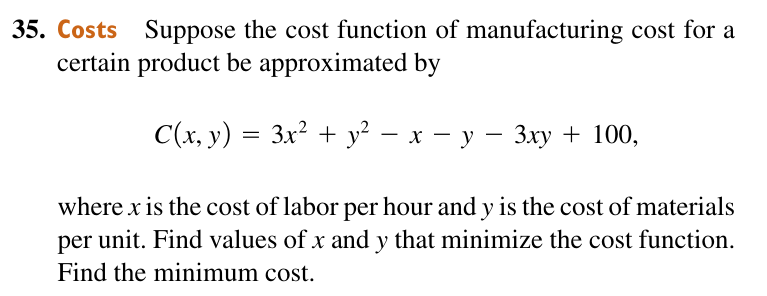
\includegraphics[width=0.96\textwidth]{screenshots/35.png}
        \end{center}
        \begin{center}
            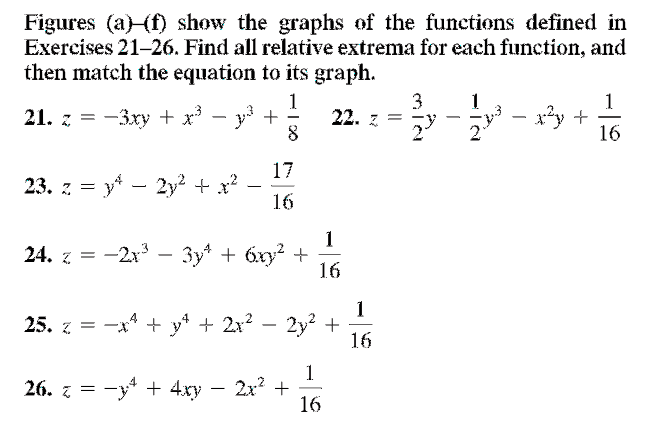
\includegraphics[width=0.96\textwidth]{screenshots/21-1.png}
            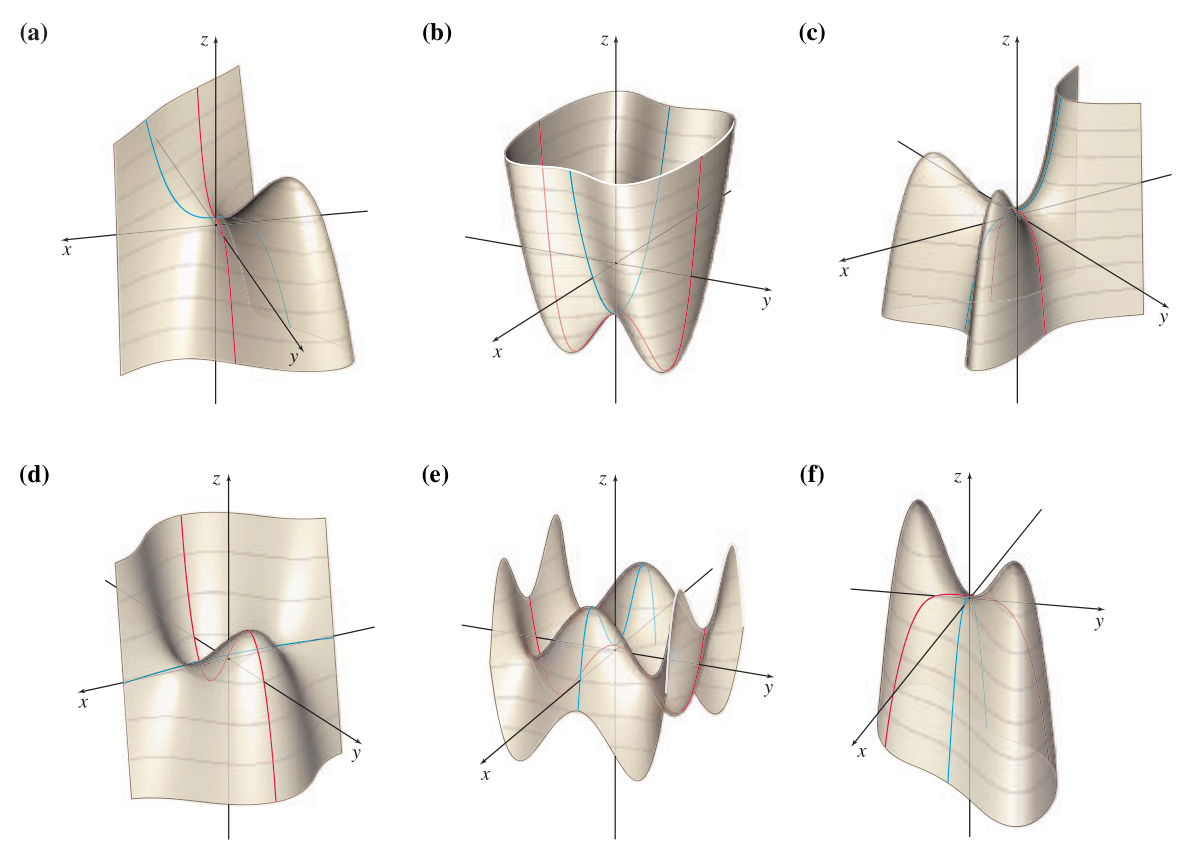
\includegraphics[width=0.96\textwidth]{screenshots/21-2.png}
        \end{center}

        \newpage

    \item 
        (\textsc{\textcolor{magenta}{Submit}})
        \begin{center}
            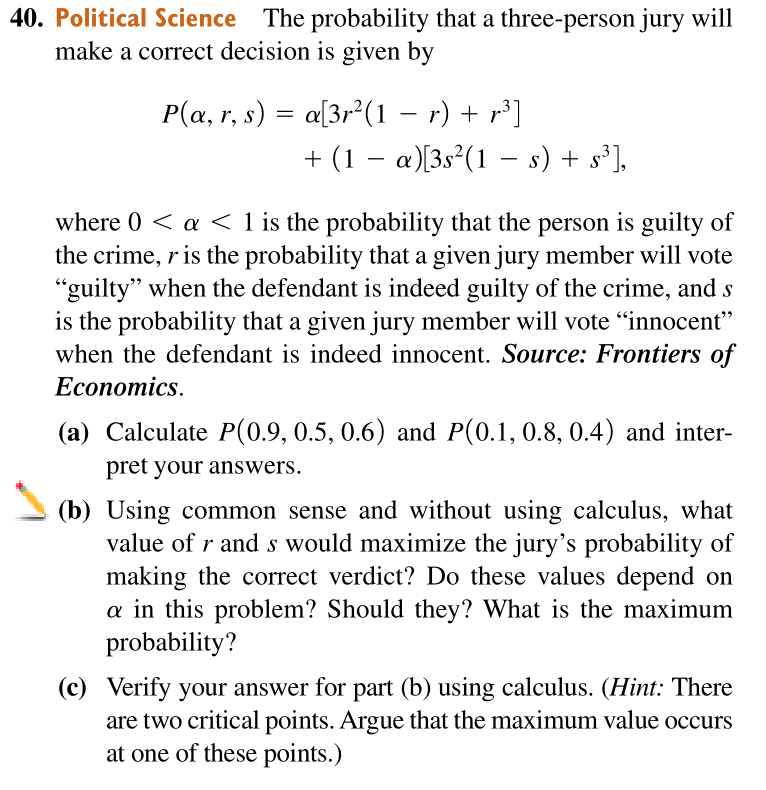
\includegraphics[width=0.96\textwidth]{screenshots/40.png}
        \end{center}

    \item 
        (\textsc{Research Maybe?})
        The hyperbolic paraboloid given by the graph of $f(x,y) = x^2-y^2$ 
        is our canonical example of a surface with a saddle point.
        We can see it has a saddle point at $(0,0)$ without even investigating
        the discriminant, by noting instead that 
        \begin{itemize}
            \item $f_x(0,0)=0$ and  $f_y(0,0)=0$, so it's``flat'' at $(0,0)$,
            \item $f_{xx}(0,0) > 0$ so it flairs upward along the $x$-axis, and
            \item $f_{yy}(0,0) < 0$ so it flairs downward along the $y$-axis.
        \end{itemize}
        Can you come up with (or find) and example of a function $g$
        that has a saddle point at a point $(a,b)$,
        but such that $g_{xx}(a,b)$ and $g_{yy}(a,b)$ are either both positive
        or both negative? Ie $(a,b)$ is a saddle point even though
        the graph of $g$ flairs in the same direction 
        along both the $x$-axis and $y$-axis?

    \item % Lagrange Multipliers
        You should become proficient at using \emph{the method %
        of Lagrange multipliers} to solve optimization problems. 
        Really this comes down to recalling what \emph{the method} entails,
        and crunching some equations.
        Just gotta practice. 
        Solve a bunch of these problems from the beginning of 
        Chapter 9.4 of \emph{Calculus with Applications, 11th Edition}.
        Also check out these exercises:
        \begin{center}
            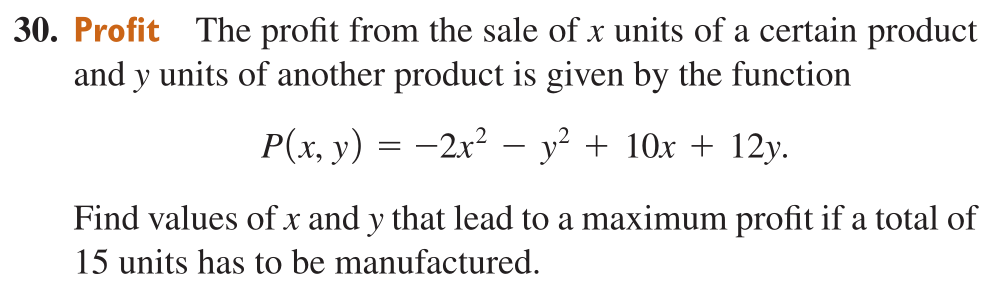
\includegraphics[width=0.96\textwidth]{screenshots/30.png}
            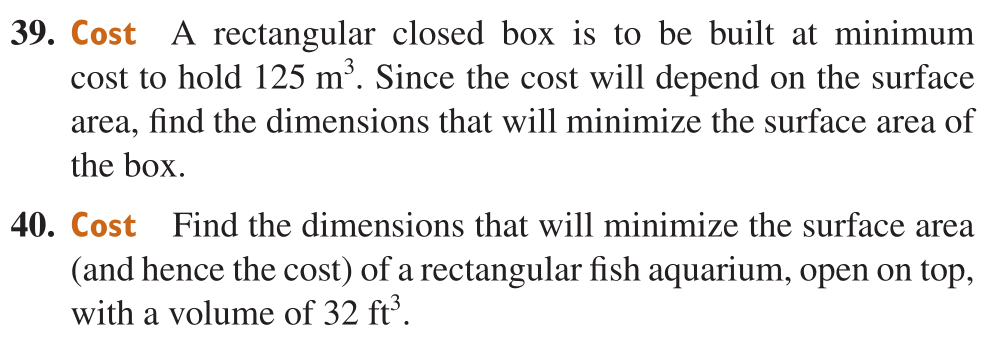
\includegraphics[width=0.96\textwidth]{screenshots/39.png}
        \end{center}

    \item
        (\textsc{\textcolor{magenta}{Submit}})
        \begin{center}
            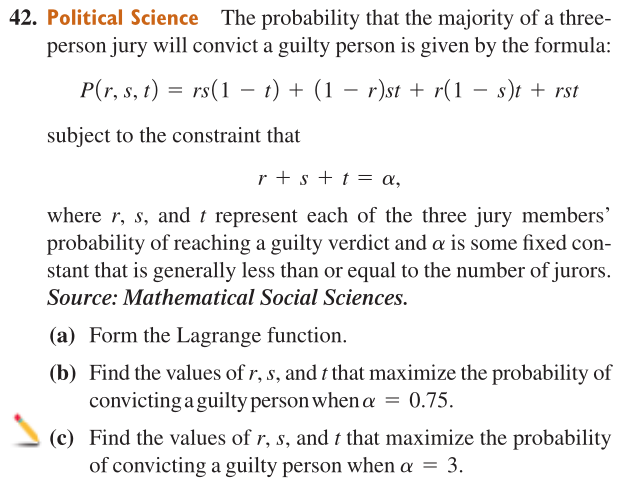
\includegraphics[width=0.96\textwidth]{screenshots/42.png}
        \end{center}

    \item % Total Differentials
        In Chapter 9.5 of \emph{Calculus with Applications, 11th Edition}
        many of the exercises are contrived. 
        I guess you should be able to wield the total differential 
        to estimate some strange numbers though.
        Work though exercises 7, 9, 11, and 13 here,
        and then \textsc{\textcolor{magenta}{Submit}} your 
        calculations for to exercise 8.
        \begin{center}
            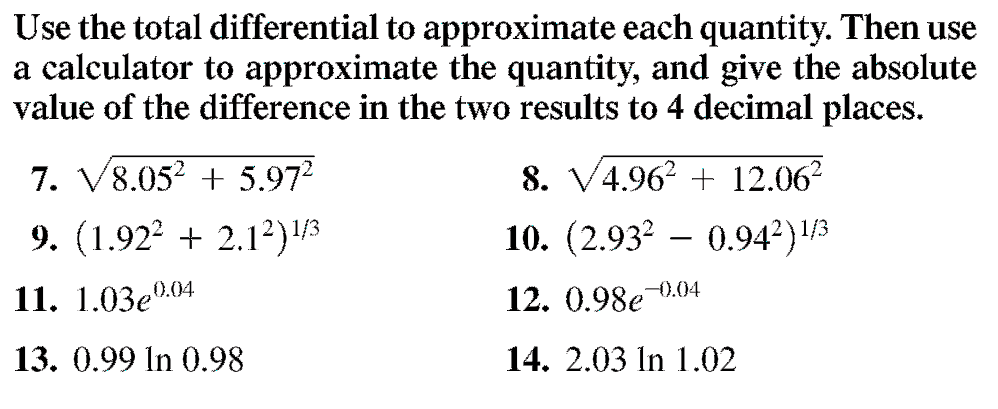
\includegraphics[width=0.96\textwidth]{screenshots/7.png}
        \end{center}

    \item 
        (\textsc{Recreation})
You are placing planes in three-dimensional space that all go through the origin $(0,0,0)$
with the goal of separating space into as many parts as possible. So when you place the first plane,
you've separated space into two pieces. You can place a second plane and separate space into four pieces,
and then you can place a third plane to separate space into eight parts (think of the coordinate planes
as an example of this). If you were to place a fourth plane in space going through the origin, 
what is the largest number of parts that you can have divided space into?
Then what if you place a fifth plane in space?

        %Three friends Anita, Becca, and Charleston 
        %are challenged to a game by the Game Maestro.
        %The Game Maestro places two colored dots 
        %on each of the friends' foreheads
        %and tells the friends that each dot is either blue or yellow,
        %but neither color is used more than four times.
        %He then places the three friends in a circle so that each of them
        %can see the dots on their friends' foreheads, but not on their own.
        %Then the game goes like this:
        %The Maestro will ask the friends in turn, 
        %first Anita, then Becca, then Charleston, then Anita again, 
        %then Becca again, and so on, 
        %if they know the colors of the dots on their foreheads.
        %If someone responds ``no,'' the Maestro asks the next person.
        %If someone responds ``yes'' and is right, the friends win!
        %Whereas if someone responds ``yes'' and is wrong, 
        %all three friends will be banished to the shadow realm.

        %The friends were given no time to strategize, 
        %but they begin playing. Their responses in turn are
        %\begin{center}
        %    no 
        %    \hspace{2ex}
        %    no 
        %    \hspace{2ex}
        %    no 
        %    \hspace{2ex}
        %    no 
        %    \hspace{2ex}
        %    yes
        %\end{center}
        %and the three friends win! 
        %Whare are the colors of the dots on Becca's forehead?

    % Five women and a monkey were shipwrecked on a desert island.
    % They spent the first day gathering coconuts for food,
    % piling up all the coconuts together 
    % before they went to sleep for the night. 
    % But while they were all asleep, one woman woke up and thought 
    % there might be a row about dividing the coconuts in the morning, 
    % so she decided to get up and take her share now. 
    % She divided the coconuts into five equal piles except for
    % one coconut left over which she gave to the monkey, 
    % and she hid her pile and put the rest back together. 
    % By and by, another woman woke up and did the same thing,
    % and similarly she had one coconut left over 
    % which she gave to the monkey. 
    % And each of the five women did the same thing, one after the other; 
    % each one taking a fifth of the coconuts in the pile when she woke up, 
    % and each one having one left over for the monkey. 
    % In the morning they divided what coconuts were left, 
    % and they came out in five equal shares. 
    % Of course each one must have known that there were coconuts missing,
    % but each one was as guilty as the others, 
    % so they didn't say anything. 
    % How many coconuts were there in the beginning?

% There's a map of the world that has every single town in the world marked on it. 
% For each town on this map you draw a straight line connecting it to its nearest neighboring town 
% (nearest in terms of distance along a straight line, <i>not</i> distance along roads).
% Show that after you've done this for every town on the map, 
% each town can be connected to at most five others.

\end{enumerate}

\end{document}

